%% Anonymous submission build (ACM sigconf, review mode).
\documentclass[sigconf,anonymous,review]{acmart}
\settopmatter{printacmref=false}
\setcopyright{none}
\renewcommand\footnotetextcopyrightpermission[1]{}
\acmConference[KDD '27]{Submitted to the 33rd ACM SIGKDD Conference on Knowledge Discovery and Data Mining}{August 2027}{San Jos\'e, CA, USA}
\acmBooktitle{}\acmDOI{}\acmISBN{}

\usepackage{booktabs}
\usepackage{multirow}
\usepackage{tikz}
\usetikzlibrary{positioning,arrows.meta,calc}
\usepackage{xspace}
\newcommand{\benchname}{PD-Bench\xspace}
\citestyle{acmauthoryear}

\begin{document}

\title{Trained Small, Scored Fairly: A 0.3M-Parameter Graph Model Against Published Specialists and
Zero-Shot Foundation Models on Physical Network Forecasting}

\author{Anonymous Authors}
\affiliation{\institution{Anonymous Institution}\country{}}

\begin{abstract}
Time-series foundation models now forecast any series zero-shot, while graph specialists are still trained per
network, and the two are rarely compared under one protocol. We compare them on physical sensor networks with a fixed,
open benchmark: six traffic networks (PEMS03/04/07/08, METR-LA, PEMS-BAY) and two monsoon rainfall regions, four
tracks (standard context, open context, 30\% dead sensors, zero-shot transfer), one scorer for point error, pinball
loss and interval score, saved forecasts and paired Diebold--Mariano and block-bootstrap tests. We introduce PWM-Dyn,
a 0.3M-parameter graph-diffusion model with explicit missing-data inputs, quantile heads and split-conformal
calibration, and compare it with STID, Graph WaveNet and STAEformer trained with their official code on identical
windows under a fixed compute budget, and with zero-shot TimesFM 2.5 and 3.0. Configurations were chosen on
validation and the reported models use fresh seeds; four networks were never used during development. Under a
12-step context PWM-Dyn has the lowest MAE on five of six traffic networks (0.3--4.2\% below the best trained opponent
on the four new ones), is statistically tied with STID on two, and trails a budget-capped STAEformer on PEMS08. Against
TimesFM 3.0 it has lower MAE and interval score on seven of eight tasks and loses on PEMS03. With 30\% of sensors dark it beats per-sensor
climatology on seven of eight tasks, where specialists without a missing-data mechanism fail. An ablation traces an earlier
accuracy loss to a climatology input. Code, benchmark and forecasts are released.
\end{abstract}

\keywords{spatio-temporal forecasting, graph neural networks, time-series foundation models, benchmarking,
probabilistic forecasting, conformal prediction, traffic, rainfall}

\maketitle

\section{Introduction}
\sloppy

Forecasting how traffic or rainfall evolves over a physical network is a long-standing data-mining task with two
competing recipes. Specialists, mostly graph neural networks and transformers, are trained on one network's
history~\citep{li2018dcrnn,wu2019graphwavenet,shao2022stid,liu2023staeformer}. Time-series foundation models such
as TimesFM~\citep{das2024timesfm} are pretrained once on large corpora and forecast any series zero-shot. Each
recipe is usually evaluated in its own protocol: specialists on point error over fixed windows, often with numbers
copied from earlier papers, and foundation models on aggregate leaderboards of unrelated series. A practitioner
choosing between them for a given network has no like-for-like evidence, and benchmark studies have shown that
re-running published specialists under one pipeline changes their rankings~\citep{shao2024basicts}.

We ask a narrow question with a fixed protocol: on real sensor networks, how does a small model trained from
scratch on the network's own history compare with (a)~published specialists run with their authors' code and
(b)~zero-shot foundation models, on the same windows, with the same point and probabilistic scores, when a third of
the sensors go dark, and with tests that say whether the differences are larger than noise?

\paragraph{Contributions.}
\begin{itemize}
\item \textbf{PWM-Dyn} (\S\ref{sec:model}), a $3\times10^5$-parameter graph-diffusion model with explicit missing-data
inputs, three quantile heads and split-conformal calibration, trained in 9--52 GPU-minutes per seed on a free T4.
\item \textbf{\benchname{}} (\S\ref{sec:bench}), an open benchmark of six traffic networks and two monsoon rainfall
regions with four tracks (standard context, open context, dead sensors, zero-shot transfer), one scorer for point,
quantile and interval quality, saved forecasts and paired significance tests.
\item \textbf{A controlled comparison} (\S\ref{sec:exp}) against STID, Graph WaveNet and STAEformer trained with
their official code and published hyper-parameters on our windows, and against TimesFM 2.5 and 3.0 zero-shot. Every
PWM-Dyn configuration choice was made on validation data and the reported models use seeds never used during
development; four of the six traffic networks were never touched during development.
\item \textbf{Findings, including losses.} Under a 12-step context a three-seed PWM-Dyn ensemble has the lowest MAE of the four trained models on five of six traffic networks and is
second on PEMS08, where STAEformer leads by 1.4\% even though its run was cut short; against STID, the
closest rival, the margins are significant on three networks and not significant on PEMS08, PEMS04
and PEMS07,
and single PWM-Dyn seeds are slightly worse than single STID runs on three networks. Against zero-shot
TimesFM~3.0 it has lower MAE on seven of eight tasks (rainfall entries from the previous version) and lower interval score on seven of eight, and loses on PEMS03.
With 30\% of sensors dark it beats per-sensor climatology on seven of eight tasks while specialists without a
missing-data mechanism fail, but climatology beats it on PEMS07. An ablation shows that a climatology input added in an earlier
version cost accuracy under the short context; removing it, chosen on validation, gave the reported model.

\end{itemize}

\section{Related work}
\label{sec:related}

\paragraph{Spatio-temporal specialists.} Traffic forecasting on sensor graphs moved from diffusion-convolutional
recurrence (DCRNN~\citep{li2018dcrnn}) and graph convolution with temporal gating (STGCN~\citep{yu2018stgcn}) to
learned adjacency (Graph WaveNet~\citep{wu2019graphwavenet}, MTGNN~\citep{wu2020mtgnn}, AGCRN~\citep{bai2020agcrn}),
attention (GMAN~\citep{zheng2020gman}, PDFormer~\citep{jiang2023pdformer}) and, recently, simple identity-embedding
models (STID~\citep{shao2022stid}) and an embedding-heavy vanilla transformer (STAEformer~\citep{liu2023staeformer}).
Benchmark studies report that gains between recent models are small and sensitive to protocol details, and that
re-running models under one pipeline changes rankings~\citep{shao2024basicts,liu2023largest}. We follow that
lesson: every opponent is run with its authors' code on our windows rather than quoted. Missing and dead sensors
are usually treated as a separate kriging problem~\citep{wu2021ignnk}; our robustness track scores it inside the
forecasting task.

\paragraph{Time-series foundation models.} TimesFM~\citep{das2024timesfm,timesfmrepo}, Chronos~\citep{ansari2024chronos},
Moirai~\citep{woo2024moirai}, Time-MoE~\citep{shi2025timemoe} and Sundial~\citep{sundial} are pretrained on large
corpora and forecast new series zero-shot, with long contexts and, in TimesFM~3.0, cross-series attention. They
are rarely compared with trained graph specialists under identical windows, metrics and uncertainty scores; this
paper does that for two TimesFM generations.

\paragraph{Uncertainty.} Quantile regression~\citep{koenker1978quantiles} with conformal
calibration~\citep{romano2019cqr} gives finite-sample coverage under exchangeability; proper scores such as
the pinball loss and the interval score~\citep{gneiting2007scoring} reward sharp, calibrated intervals. Traffic
benchmarks almost always report point metrics only.

\section{PWM-Dyn}
\label{sec:model}

\paragraph{Problem.} A network has $N$ locations (road sensors or grid cells) joined by a fixed physical
graph $A\in\mathbb{R}^{N\times N}$ built from road distance or geographic adjacency. From the last $L$ observations
$X\in\mathbb{R}^{L\times N}$, an observed-mask $O\in\{0,1\}^{L\times N}$ (0 = no reading), the position $p$ of the last
step in its daily or yearly cycle and the day of week $w$, the model returns three quantiles for each of the next $H$
steps and every location,
\begin{equation}
\hat Q = f_\theta(X, O, p, w, A, C)\in\mathbb{R}^{H\times N\times 3},\qquad \hat Q_{h,n,1}\le\hat Q_{h,n,2}\le\hat Q_{h,n,3},
\end{equation}
the 10th, 50th and 90th percentiles. $C\in\mathbb{R}^{H\times N}$ is the training-split climatology of the
forecast steps: the per-location median at the same time of week (traffic, $\pm 5$ minutes) or day of year
(rainfall, $\pm 7$ days), computed once from the training split. The median is the point forecast and
$[\hat Q_{\cdot,\cdot,1},\hat Q_{\cdot,\cdot,3}]$ the 80\% prediction interval.

\paragraph{Architecture.} PWM-Dyn (Figure~\ref{fig:arch}) gives every location a $d{=}96$-dimensional state and mixes
it with its physical neighbours. (i)~A two-layer MLP reads the location's history concatenated with its mask,
$[X\odot O;\,O]$, so a missing reading is an explicit zero flag rather than an imputed value; four scale-free cues
(last value, masked mean, trend, observed share) enter through a separate linear map. (ii)~Learned embeddings of
$p$ and $w$ are added to every location. (iii)~Optionally, a linear map of $C$ is added. (iv)~In the transductive variant, a
per-location embedding and a learned low-rank graph $G=\mathrm{softmax}(\mathrm{relu}(SD^\top))$, $S,D\in\mathbb{R}^{N\times 16}$,
are added; the inductive variant drops both so its weights run on unseen networks. (v)~Three GraphMix blocks
apply two-hop diffusion over $A$ (and $G$), $h\leftarrow\mathrm{LN}(h+W[h;Ah;A^2h;Gh;G^2h])$, followed by a
residual feed-forward layer. (vi)~A linear head emits $H\times 3$ offsets from a base value and the outputs are sorted.
The base is the last observed value; when the climatology input is used and a location's last reading is missing,
the base is $C$, so a dark sensor is forecast as a deviation from its own normal pattern rather than from zero.
Whether to use $C$ is a configuration choice made on validation (\S\ref{sec:exp}): the reported standard-context
model omits it and the long-context variant keeps it. The transductive model has $3.2\times10^5$ parameters on PEMS08.

\paragraph{Training.} From random initialisation, with the pinball loss on the three quantiles plus an $L_1$ term on
the median, over valid targets only (missing and zero readings excluded on traffic, as in the literature).
During training each batch hides a random share $r\sim U(0, 0.3)$ of locations for the whole input window,
which forces the model to reconstruct them from their neighbours. AdamW (weight decay $10^{-4}$), one-cycle schedule with peak learning rate $2\times10^{-3}$, batch 32, gradient
clipping at 5, a fixed budget of $\approx$33.5k optimisation steps (100 epochs on PEMS08); the checkpoint with the
lowest validation MAE is kept.

\paragraph{Long-context variant.} For the open-context track the input also carries the 24 values around the same
time one day earlier (traffic) or the same week one year earlier (rainfall); total look-back 300 steps or 365 days,
inside the foundation models' budget. Whether a task uses it is decided on validation.

\paragraph{Calibration.} Quantile losses alone under-cover on heavy-tailed targets. We apply split-conformal
quantile regression~\citep{romano2019cqr} on the validation split: per horizon, the score
$s=\max(\hat Q_1-y,\,y-\hat Q_3)$ in the model's target space gives an offset $\delta_h$ (its $\lceil (n+1)0.8\rceil/n$
quantile), and the test interval becomes $[\hat Q_1-\delta_h,\hat Q_3+\delta_h]$. The median, hence MAE and RMSE,
is unchanged. Each reported PWM-Dyn entry is the quantile mean of three independently trained seeds.


\begin{figure*}[t]
\centering
\resizebox{0.92\textwidth}{!}{% Figure 1: PWM-Dyn forward pass (vector, TikZ)
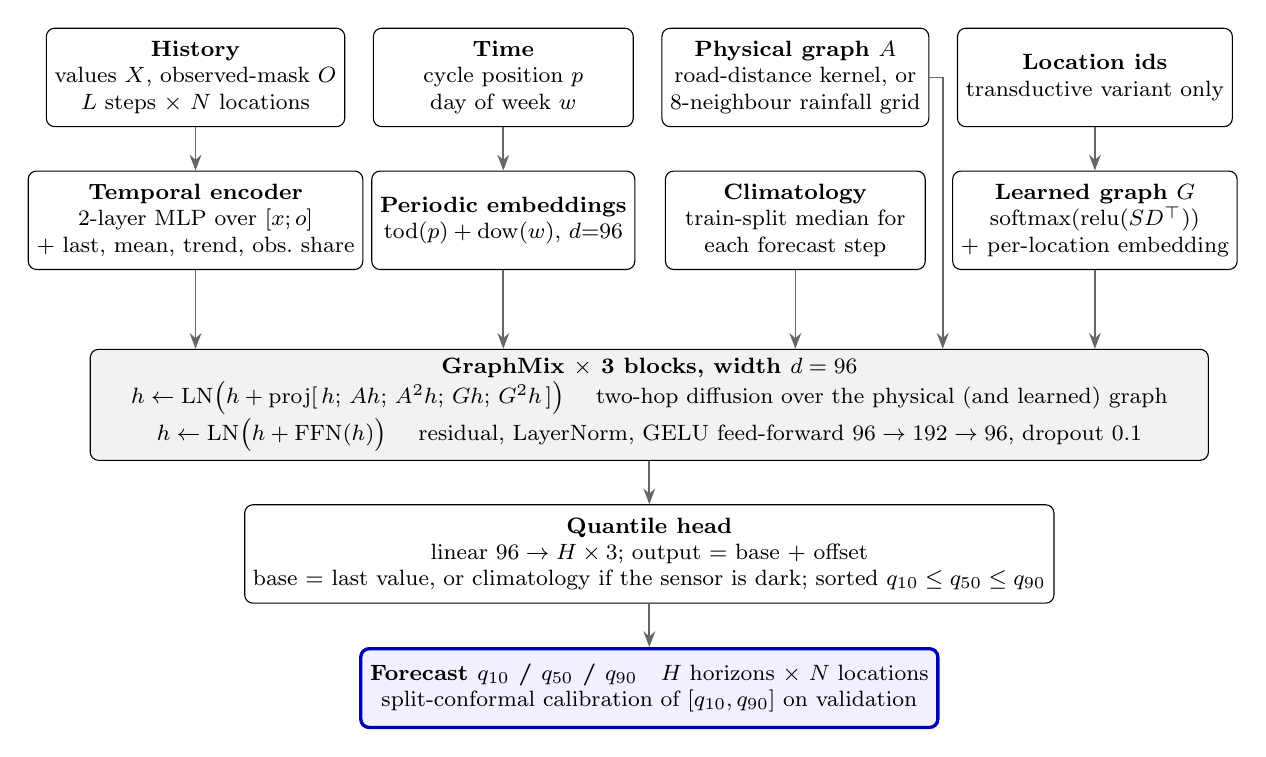
\begin{tikzpicture}[
  font=\footnotesize,
  box/.style={draw, rounded corners=3pt, align=center, minimum width=3.3cm, minimum height=1.25cm, inner sep=3pt},
  wide/.style={draw, rounded corners=3pt, align=center, fill=black!5, minimum width=14.2cm, minimum height=1.25cm, inner sep=3pt},
  fcst/.style={draw=blue!70!black, very thick, rounded corners=3pt, align=center, fill=blue!6, minimum width=6.6cm, minimum height=1.0cm},
  arr/.style={-{Stealth[length=2mm]}, semithick, draw=black!60},
  node distance=0.55cm and 0.35cm]
  % inputs
  \node[box] (hist)  {\textbf{History}\\values $X$, observed-mask $O$\\$L$ steps $\times$ $N$ locations};
  \node[box, right=of hist] (time) {\textbf{Time}\\cycle position $p$\\day of week $w$};
  \node[box, right=of time] (graph) {\textbf{Physical graph $A$}\\road-distance kernel, or\\8-neighbour rainfall grid};
  \node[box, right=of graph] (ids) {\textbf{Location ids}\\transductive variant only};
  % encoders
  \node[box, below=of hist] (tenc) {\textbf{Temporal encoder}\\2-layer MLP over $[x;o]$\\+ last, mean, trend, obs.\ share};
  \node[box, below=of time] (per)  {\textbf{Periodic embeddings}\\$\mathrm{tod}(p)+\mathrm{dow}(w)$, $d{=}96$};
  \node[box, below=of graph] (clim) {\textbf{Climatology}\\train-split median for\\each forecast step};
  \node[box, below=of ids] (lg)   {\textbf{Learned graph $G$}\\$\mathrm{softmax}(\mathrm{relu}(SD^\top))$\\+ per-location embedding};
  % graphmix
  \node[wide, below=1.0cm of $(per.south)!0.5!(clim.south)$] (gm)
    {\textbf{GraphMix $\times$ 3 blocks, width $d=96$}\\
     $h \leftarrow \mathrm{LN}\big(h + \mathrm{proj}[\,h;\,Ah;\,A^2h;\,Gh;\,G^2h\,]\big)$ \quad two-hop diffusion over the physical (and learned) graph\\
     $h \leftarrow \mathrm{LN}\big(h + \mathrm{FFN}(h)\big)$ \quad residual, LayerNorm, GELU feed-forward $96\to192\to96$, dropout 0.1};
  \node[box, below=of gm, minimum width=6.6cm] (head) {\textbf{Quantile head}\\linear $96 \to H\times 3$; output = base + offset\\base = last value, or climatology if the sensor is dark; sorted $q_{10}\le q_{50}\le q_{90}$};
  \node[fcst, below=of head] (fc) {\textbf{Forecast $q_{10}$ / $q_{50}$ / $q_{90}$}\quad $H$ horizons $\times$ $N$ locations\\split-conformal calibration of $[q_{10}, q_{90}]$ on validation};
  % arrows
  \draw[arr] (hist) -- (tenc);
  \draw[arr] (time) -- (per);
  \draw[arr] (ids) -- (lg);
  \draw[arr] (tenc) -- (tenc |- gm.north);
  \draw[arr] (per) -- (per |- gm.north);
  \draw[arr] (clim) -- (clim |- gm.north);
  \draw[arr] (lg) -- (lg |- gm.north);
  \draw[arr] (graph.east) -- ++(0.17,0) -- ($(gm.north -| graph.east)+(0.17,0)$);
  \draw[arr] (gm) -- (head);
  \draw[arr] (head) -- (fc);
\end{tikzpicture}
}
\caption{PWM-Dyn. Each location's history and observed-mask, the time, the training-split climatology and (in the
transductive variant) a location embedding form a state that three GraphMix blocks diffuse over the physical
graph $A$ and a learned graph $G$; a linear head returns three quantiles per horizon as offsets from the last
reading, or from climatology when the sensor is dark.}
\label{fig:arch}
\end{figure*}

\section{The \benchname{} benchmark}
\label{sec:bench}

\benchname{} scores every model, specialist or foundation model, with one function on frozen windows. Version
1.1, used here, has ten tasks (Table~\ref{tab:tasks}): six traffic networks with their standard literature
protocols (12 five-minute steps in, 12 out; chronological 60/20/20 split for PeMS flow, 70/10/20 for the two
speed datasets) and two Indian monsoon rainfall regions from the IMD $0.25^\circ$ daily grid~\citep{nandi2024imdlib}
(30 days in, 7 out; 2000--2018 train, 2019--2021 validation, 2022--2024 test). Values and time features of the
four tasks added in 1.1 come from public copies of the datasets and road graphs from the DCRNN and ASTGNN
releases~\citep{li2018dcrnn,guo2019astgcn}; a script rebuilds them, so nothing is re-hosted.

\begin{table}[t]
\caption{\benchname{}-1.1 tasks. Windows: official test windows (every 2nd; every 6th on the four tasks added in
1.1, so that foundation models fit a free-GPU budget). All models on a task are scored on the same windows.}
\label{tab:tasks}
\scriptsize
\setlength{\tabcolsep}{3pt}
\begin{tabular}{@{}llrrl@{}}
\toprule
Task & Quantity & $N$ & Steps & Windows \\
\midrule
PEMS08 / PEMS04 & flow, veh/5 min & 170 / 307 & 17,856 / 16,992 & 1,775 / 1,688 \\
PEMS03 / PEMS07 & flow, veh/5 min & 358 / 883 & 26,208 / 28,224 & 870 / 937 \\
METR-LA / PEMS-BAY & speed, mph & 207 / 325 & 34,272 / 52,116 & 1,139 / 1,734 \\
IMD-CI / IMD-WC & rain, mm/day & land cells & 9,132 days & 530 / 530 \\
\bottomrule
\end{tabular}
\end{table}

\paragraph{Tracks.} \textbf{A (standard)}: look-back limited to the standard context (12 steps, 30 days); any
training on the task's training split. \textbf{B (open context)}: look-back up to 512 steps or 365 days;
foundation models run zero-shot here. \textbf{R (dead sensors)}: 30\% of locations, fixed by a seeded
permutation, have no observations during the test period and are scored on those locations only.
\textbf{Z (transfer)}: forecast PEMS08 with a model that has seen no PEMS08 data, not even its normalisation
statistics or validation split.

\paragraph{Metrics.} MAE, RMSE and MAPE of the median; QL, the mean pinball loss over the three quantiles (a proper
score; $2\,\mathrm{QL}$ approximates CRPS); IS80, the interval score~\citep{gneiting2007scoring} of the 80\% interval
(width plus $10\times$ the size of any miss); and COV80, the share of truths inside it. MAE is the headline point
metric and IS80 the headline uncertainty metric; point-only models report MAE, RMSE and MAPE.

\paragraph{Protocol.} Test data may not be used for training, selection, early stopping or calibration;
validation data may. Each scored entry keeps its forecast file, so any two entries can be compared on the same
windows. Paired comparisons use the Diebold--Mariano test~\citep{diebold1995dm} on per-window absolute-error
differences with a Newey--West~\citep{newey1987hac} long-run variance (one-day bandwidth), and a moving-block
bootstrap~\citep{kunsch1989bootstrap} over whole days (2,000 resamples) for a 95\% interval on the relative MAE
difference.

\section{Experiments}
\label{sec:exp}

\paragraph{Models.} \emph{Specialists}: STID~\citep{shao2022stid}, Graph WaveNet~\citep{wu2019graphwavenet} and
STAEformer~\citep{liu2023staeformer}, imported unchanged from their official repositories (pinned commits in the
supplement) and trained on each task's training split with the published hyper-parameters, loss, optimiser,
schedule and early stopping, on exactly the windows PWM-Dyn uses. The one code change is a compatibility fix in Graph
WaveNet, whose 2-D-kernel \texttt{Conv1d} layers are rejected by current PyTorch and are built as \texttt{Conv2d}, the
operation they computed. Each run had a wall-clock budget on one T4 (Table~\ref{tab:budget}); runs that hit it keep
their best-validation checkpoint and are marked. \emph{Foundation models}: TimesFM~2.5 (200M) and TimesFM~3.0 in its
multivariate mode, zero-shot, with a 512-step (365-day) context, run in a separate software environment.
\emph{References}: last value, seasonal naive and per-location climatology quantiles from the training split.
\emph{PWM-Dyn}: the configuration frozen by the ablation below, three fresh seeds (100--102), trained for the
optimisation-step budget it has on PEMS08 ($\approx$33.5k steps; 9--52 GPU-minutes per seed), conformally
calibrated on validation and scored once.

\begin{table*}[t]
\caption{Point accuracy: test MAE (RMSE below) on the official windows. Upper block: Track A, 12-step context, every model trained on the task's training split; lower block: Track B, foundation models zero-shot with 512 steps (365 days on rainfall). Bold: best MAE in the block. $^\dagger$\,stopped by its wall-clock budget before its authors' schedule ended (Table~\ref{tab:budget}). $^\ast$\,network never used during development. Rainfall PWM-Dyn entries are v0.4; rainfall has no specialist entries. Units: vehicles/5\,min (PeMS flow), mph (METR-LA, PEMS-BAY), mm/day (IMD).}
\label{tab:main}
\small
\setlength{\tabcolsep}{4pt}
\begin{tabular}{@{}lrrrrrrrr@{}}
\toprule
Model & PEMS08 & PEMS04 & PEMS03$^\ast$ & PEMS07$^\ast$ & METR-LA$^\ast$ & PEMS-BAY$^\ast$ & IMD-CI & IMD-WC \\
\midrule
Last value & 25.30 & 31.56 & 23.89 & 35.63 & 5.04 & 2.17 & 4.37 & 4.88 \\
 & {\scriptsize 38.66} & {\scriptsize 48.25} & {\scriptsize 37.31} & {\scriptsize 54.37} & {\scriptsize 10.98} & {\scriptsize 5.11} & {\scriptsize 13.55} & {\scriptsize 14.94} \\[1pt]
Climatology & 22.18 & 25.02 & 25.93 & 29.98 & 3.90 & 2.53 & 2.89 & 3.65 \\
 & {\scriptsize 40.77} & {\scriptsize 41.36} & {\scriptsize 47.80} & {\scriptsize 58.67} & {\scriptsize 8.41} & {\scriptsize 5.48} & {\scriptsize 10.70} & {\scriptsize 13.00} \\[1pt]
\midrule
STID & 14.18 & 18.49 & 15.50 & 19.62$^\dagger$ & 3.12 & 1.56$^\dagger$ & -- & -- \\
 & {\scriptsize 23.21} & {\scriptsize 30.05} & {\scriptsize 26.83} & {\scriptsize 32.72} & {\scriptsize 6.50} & {\scriptsize 3.60} &  &  \\[1pt]
Graph WaveNet & 14.77 & 19.37$^\dagger$ & 14.70$^\dagger$ & 23.39$^\dagger$ & 3.05$^\dagger$ & 1.57$^\dagger$ & -- & -- \\
 & {\scriptsize 23.59} & {\scriptsize 30.75} & {\scriptsize 25.17} & {\scriptsize 36.92} & {\scriptsize 6.15} & {\scriptsize 3.57} &  &  \\[1pt]
STAEformer & \textbf{13.93}$^\dagger$ & 19.21$^\dagger$ & 15.45$^\dagger$ & -- & 3.09$^\dagger$ & 1.59$^\dagger$ & -- & -- \\
 & {\scriptsize 23.17} & {\scriptsize 30.66} & {\scriptsize 26.03} &  & {\scriptsize 6.33} & {\scriptsize 3.63} &  &  \\[1pt]
PWM-Dyn (ours) & 14.12 & \textbf{18.46} & \textbf{14.34} & \textbf{19.56} & \textbf{2.92} & \textbf{1.52} & \textbf{2.84} & \textbf{3.41} \\
 & {\scriptsize 23.46} & {\scriptsize 30.77} & {\scriptsize 23.12} & {\scriptsize 32.60} & {\scriptsize 5.88} & {\scriptsize 3.45} & {\scriptsize 10.42} & {\scriptsize 12.01} \\[1pt]
\midrule
TimesFM 2.5 & 15.04 & 19.70 & -- & -- & -- & -- & 2.96 & 3.67 \\
 & {\scriptsize 24.09} & {\scriptsize 31.70} &  &  &  &  & {\scriptsize 10.58} & {\scriptsize 12.65} \\[1pt]
TimesFM 3.0 mv & 14.55 & 19.13 & \textbf{14.15} & 20.27 & 3.40 & 1.66 & 2.92 & 3.62 \\
 & {\scriptsize 23.57} & {\scriptsize 31.02} & {\scriptsize 22.70} & {\scriptsize 33.13} & {\scriptsize 6.97} & {\scriptsize 3.95} & {\scriptsize 10.65} & {\scriptsize 12.78} \\[1pt]
PWM-Dyn (ours), Track B & \textbf{14.18} & \textbf{18.46} & 14.34 & \textbf{19.56} & \textbf{2.92} & \textbf{1.52} & \textbf{2.84} & \textbf{3.41} \\
 & {\scriptsize 23.38} & {\scriptsize 30.77} & {\scriptsize 23.12} & {\scriptsize 32.60} & {\scriptsize 5.88} & {\scriptsize 3.45} & {\scriptsize 10.42} & {\scriptsize 12.01} \\[1pt]
\bottomrule
\end{tabular}
\end{table*}

\subsection{Point accuracy}
Table~\ref{tab:main} gives test MAE and RMSE. Under the standard 12-step context (upper block) PWM-Dyn has the lowest
MAE on PEMS04, PEMS03, PEMS07, METR-LA and PEMS-BAY and is second on PEMS08 (14.12) behind STAEformer (13.93), which
reached only 25 of its scheduled epochs; STAEformer's published PEMS08 result, 13.46 on all test windows, is better
still. On the four networks never used during development the margin over the best opponent is 2.5\% (PEMS03, Graph
WaveNet), 0.3\% (PEMS07, STID), 4.2\% (METR-LA, Graph WaveNet) and 2.7\% (PEMS-BAY, STID). STID, the only opponent
that completed its authors' schedule on most networks, is PWM-Dyn's closest rival everywhere and essentially ties it on
PEMS08 and PEMS04. In the open-context block, TimesFM~3.0 run zero-shot beats every specialist trained with our
budget on PEMS03 (14.15) and is ahead of or within 4\% of PWM-Dyn on four of six traffic networks; PWM-Dyn's long-context variant
was preferred on validation only for PEMS08. RMSE orders the models similarly, with exceptions: all three specialists on PEMS04, and STID and STAEformer on
PEMS08, have lower RMSE than PWM-Dyn, i.e.\ smaller errors on the largest deviations.


\subsection{Is the difference larger than noise?}
\begin{table}[t]
\caption{Paired tests of PWM-Dyn against each model on the same windows: relative MAE difference (negative = PWM-Dyn better) and Diebold--Mariano $p$-value; in brackets the 95\% day-block bootstrap interval. Track A for specialists, Track B for TimesFM. $^\dagger$\,opponent budget-capped.}
\label{tab:sig}
\scriptsize
\setlength{\tabcolsep}{2.5pt}
\begin{tabular}{@{}lcccc@{}}
\toprule
Task & STID & GWNet & STAEf. & TimesFM 3.0 \\
\midrule
PEMS08 & \shortstack{$-0.4\%$, $p=0.12$\\{}[-1.0, +0.1]} & \shortstack{$-4.4\%$, $p<10^{-3}$\\{}[-4.9, -4.0]} & \shortstack{$+1.4\%$, $p<10^{-3}$$^\dagger$\\{}[+0.7, +1.9]} & \shortstack{$-2.5\%$, $p=0.06$\\{}[-5.4, -0.3]} \\[2pt]
PEMS04 & \shortstack{$-0.2\%$, $p=0.82$\\{}[-2.0, +1.1]} & \shortstack{$-4.7\%$, $p<10^{-3}$$^\dagger$\\{}[-5.3, -4.3]} & \shortstack{$-3.9\%$, $p<10^{-3}$$^\dagger$\\{}[-4.7, -3.5]} & \shortstack{$-3.5\%$, $p=0.03$\\{}[-7.0, -0.8]} \\[2pt]
PEMS03$^\ast$ & \shortstack{$-7.5\%$, $p=0.02$\\{}[-14.1, -2.3]} & \shortstack{$-2.5\%$, $p<10^{-3}$$^\dagger$\\{}[-3.3, -1.2]} & \shortstack{$-7.2\%$, $p<10^{-3}$$^\dagger$\\{}[-10.8, -4.6]} & \shortstack{$+1.3\%$, $p=0.48$\\{}[-1.8, +5.3]} \\[2pt]
PEMS07$^\ast$ & \shortstack{$-0.3\%$, $p=0.03$$^\dagger$\\{}[-0.5, +0.0]} & \shortstack{$-16.4\%$, $p<10^{-3}$$^\dagger$\\{}[-17.5, -15.4]} & -- & \shortstack{$-3.5\%$, $p<10^{-3}$\\{}[-5.4, -1.6]} \\[2pt]
METR-LA$^\ast$ & \shortstack{$-6.6\%$, $p<10^{-3}$\\{}[-7.6, -5.5]} & \shortstack{$-4.2\%$, $p<10^{-3}$$^\dagger$\\{}[-5.0, -3.3]} & \shortstack{$-5.5\%$, $p<10^{-3}$$^\dagger$\\{}[-6.2, -4.8]} & \shortstack{$-14.2\%$, $p<10^{-3}$\\{}[-16.3, -11.5]} \\[2pt]
PEMS-BAY$^\ast$ & \shortstack{$-2.7\%$, $p<10^{-3}$$^\dagger$\\{}[-3.6, -1.9]} & \shortstack{$-3.2\%$, $p<10^{-3}$$^\dagger$\\{}[-3.9, -2.2]} & \shortstack{$-4.7\%$, $p<10^{-3}$$^\dagger$\\{}[-5.2, -4.2]} & \shortstack{$-8.5\%$, $p<10^{-3}$\\{}[-11.4, -5.2]} \\[2pt]
\bottomrule
\end{tabular}
\end{table}
Table~\ref{tab:sig} tests each comparison on the per-window error differences. Against STID, PWM-Dyn's advantage is
significant on METR-LA, PEMS-BAY and PEMS03 ($p\le0.02$; on PEMS03 the day-block interval is wide because the test
period contains Thanksgiving week), borderline on PEMS07 ($-0.3\%$, interval touching zero) and absent on PEMS08 and
PEMS04 ($p=0.12$ and $0.82$): there, the two models are statistically tied. The deficit to STAEformer on PEMS08 is
significant. Against TimesFM~3.0 the advantage is significant on PEMS04, PEMS07, METR-LA and PEMS-BAY; on PEMS08 the
bootstrap interval excludes zero but the Diebold--Mariano test does not reject ($p=0.06$); on PEMS03 TimesFM is
ahead by 1.3\%, not significantly. Seed variation is small relative to these gaps (Table~\ref{tab:abl}, right): the
standard deviation of single-seed test MAE is 0.002--0.22, and the ensemble beats every one of its seeds on every
network.


\subsection{Uncertainty and dead sensors}
\begin{table}[t]
\caption{Probabilistic quality (Track B, IS80 with 80\% coverage) and dead sensors (Track R, MAE on the 30\% of locations with no test-period readings). Specialists without a missing-data mechanism are fed zeros, their repositories' missing-value convention.}
\label{tab:prob}
\small
\setlength{\tabcolsep}{3pt}
\begin{tabular}{@{}lrrrrr@{}}
\toprule
 & \multicolumn{3}{c}{IS80 (coverage \%)} & \multicolumn{2}{c}{Track R MAE} \\
\cmidrule(lr){2-4}\cmidrule(l){5-6}
Task & PWM-Dyn & TimesFM 3.0 & Climat. & PWM-Dyn & best other \\
\midrule
PEMS08 & 66.94 (80) & 67.84 (81) & 117.83 (71) & \textbf{19.25} & 21.78\,{\scriptsize(clim.)} \\
PEMS04 & 86.23 (80) & 88.42 (81) & 127.81 (72) & \textbf{25.33} & 27.39\,{\scriptsize(clim.)} \\
PEMS03$^\ast$ & 67.14 (78) & 65.50 (81) & 154.10 (61) & \textbf{17.71} & 23.31\,{\scriptsize(clim.)} \\
PEMS07$^\ast$ & 93.99 (80) & 95.32 (81) & 159.70 (76) & 30.95 & \textbf{29.10}\,{\scriptsize(clim.)} \\
METR-LA$^\ast$ & 14.34 (81) & 17.37 (81) & 19.42 (75) & \textbf{3.36} & 4.07\,{\scriptsize(clim.)} \\
PEMS-BAY$^\ast$ & 7.54 (79) & 8.29 (81) & 13.19 (75) & \textbf{2.31} & 2.71\,{\scriptsize(clim.)} \\
IMD-CI & 18.01 (85) & 19.79 (86) & 18.21 (91) & \textbf{2.84} & 2.88\,{\scriptsize(clim.)} \\
IMD-WC & 20.27 (83) & 21.85 (87) & 21.09 (91) & \textbf{3.43} & 3.60\,{\scriptsize(clim.)} \\
\bottomrule
\end{tabular}
\end{table}
\textbf{Intervals.} After conformal calibration, PWM-Dyn's 80\% intervals cover 78--85\% of test values and have a
lower interval score than TimesFM~3.0's on seven of eight tasks (Table~\ref{tab:prob}); the exception is again
PEMS03, where TimesFM's intervals are both narrower and better covering. TimesFM's intervals slightly over-cover
(81--87\%) everywhere; climatology intervals are wide and under-cover on traffic. Specialists give point forecasts only.
\textbf{Dead sensors.} With 30\% of locations dark throughout the test period, PWM-Dyn's MAE on those locations rises
by 15--58\% over its normal accuracy on traffic (and hardly at all on rainfall) but stays below per-sensor
climatology on seven of eight tasks; on PEMS07 it is
6\% worse than climatology. The frozen configuration has no climatology fallback, the likely reason: the previous version, which has it, was
slightly better on dark sensors on PEMS08 and PEMS04 (18.70 and 24.99 against 19.25 and 25.33). The three specialists, fed zeros for the missing readings as their repositories do, produce errors of
5--310 (appendix): forecasting dark sensors needs an explicit mechanism, not just a graph.


\subsection{What cost v0.4 its accuracy}
\begin{table}[t]
\caption{Left: what cost v0.4 accuracy. Validation MAE (selection criterion, seeds 0--1) and test MAE of each configuration's ensemble; the frozen choice is marked. Right: test MAE of the three fresh seeds of the frozen model and of their ensemble (Track A). The v0.4.1 row is its own three-seed run (seeds 0--2).}
\label{tab:abl}
\scriptsize
\setlength{\tabcolsep}{2.5pt}
\begin{tabular}{@{}lrrrr@{}}
\toprule
Configuration & \multicolumn{2}{c}{Val.\ MAE} & \multicolumn{2}{c}{Test MAE} \\
\cmidrule(lr){2-3}\cmidrule(l){4-5}
 & P08 & P04 & P08 & P04 \\
\midrule
clim., 100 ep., select every 4th (v0.4.1) & 14.52 & 18.84 & 14.50 & 19.02 \\
clim., 100 ep., select every window & 14.45 & 18.84 & 14.45 & 19.06 \\
no clim., 60 ep., select every window & 14.60 & 18.61 & 14.23 & 18.47 \\
no clim., 100 ep., select every window (frozen) & 14.61 & 18.39 & 14.14 & 18.42 \\
\bottomrule
\end{tabular}
\vspace{4pt}
\begin{tabular}{@{}lrrr@{}}
\toprule
Task & Seeds (test MAE) & Mean $\pm$ SD & Ens. \\
\midrule
PEMS08 & 14.22 / 14.24 / 14.52 & 14.33 $\pm$ 0.17 & 14.12 \\
PEMS04 & 18.52 / 18.70 / 18.65 & 18.62 $\pm$ 0.09 & 18.46 \\
PEMS03$^\ast$ & 14.45 / 14.45 / 14.65 & 14.52 $\pm$ 0.12 & 14.34 \\
PEMS07$^\ast$ & 20.12 / 19.69 / 19.83 & 19.88 $\pm$ 0.22 & 19.56 \\
METR-LA$^\ast$ & 2.960 / 2.959 / 2.956 & 2.958 $\pm$ 0.002 & 2.919 \\
PEMS-BAY$^\ast$ & 1.544 / 1.536 / 1.535 & 1.538 $\pm$ 0.005 & 1.519 \\
\bottomrule
\end{tabular}
\end{table}
An earlier version of PWM-Dyn added a per-location climatology input and its test MAE under the 12-step context was
2--3\% worse than the version before it. Table~\ref{tab:abl} separates the three changes involved on validation. The
climatology input is the culprit: with it, PEMS04 validation MAE is 18.84 whichever checkpoint rule is used; without
it, 18.40--18.61. Training length and checkpoint selection matter far less. The configuration with the lowest
validation MAE averaged over both networks (no climatology input, 100 epochs, checkpoint chosen on every validation
window) was frozen before any test scoring. Its test MAE, reported for the record, is also the lowest of the four;
but on PEMS08 alone validation preferred a configuration with the climatology input, so the selection rule is not
uniformly decisive at this resolution. The climatology input is not useless: it is what makes dark sensors
forecastable, and it remains in the long-context variant.


\subsection{Cost}
PWM-Dyn has 0.32--0.41M parameters, against 0.12--0.14M (STID), 0.31--0.32M (Graph WaveNet), 1.2--1.9M (STAEformer)
and 200M (TimesFM~2.5). One seed trains in 9 (PEMS08), 9 (METR-LA), 13 (PEMS04), 14 (PEMS-BAY), 17 (PEMS03) and 52
(PEMS07) minutes on a T4, so the three-seed ensembles cost 0.4--2.6 GPU-hours per network; TimesFM~3.0 needed
0.6--2.0 GPU-hours per network for inference alone at our window counts. The study reported here ran on free Kaggle T4 GPUs in about 11
GPU-hours.


\section{Limitations}
\label{sec:limits}

\textbf{Compute-capped opponents.} Each opponent run had a fixed wall-clock budget on one T4 (30--55 minutes for
STAEformer and Graph WaveNet, 6--12 for STID; Table~\ref{tab:budget}). STID reached its authors' 100-epoch schedule
on four networks; Graph WaveNet on one; STAEformer on none, and it ran out of memory on PEMS07 at its published batch
size. The comparison is therefore compute-matched rather than converged: STAEformer's numbers in particular
understate what it reaches with its full schedule, and its published results (e.g.\ 13.46 MAE on PEMS08 with all test
windows) remain ahead of ours where reported. Each opponent was run with one seed.

\textbf{Development exposure.} PEMS08 and PEMS04 shaped PWM-Dyn's design in earlier versions, including one look at
PEMS08 test scores of development checkpoints; the reported models use fresh seeds and a configuration chosen on
validation, but the design itself is not blind on those two networks. PEMS03, PEMS07, METR-LA and PEMS-BAY were never
used during development.

\textbf{Scope.} Traffic tasks use the 12-step literature protocol and the new tasks score every sixth window.
Rainfall covers two Indian regions and its PWM-Dyn entries come from the previous model version. TimesFM 3.0 is used
zero-shot under a non-commercial research licence; we did not fine-tune it, and fine-tuned foundation models may
close the gap we report. A PWM-Dyn win over a foundation model is a specialist-versus-zero-shot result, not evidence
of better generalisation; the transfer track shows the opposite.

\section{Conclusion}

Trained on a network's own history and scored on identical windows, a $3\times10^5$-parameter graph model with
explicit missing-data inputs and conformal intervals is the most accurate of the trained models we ran on five of six traffic networks, ties the best fully trained
specialist on two of them, and beats a 2026 zero-shot foundation model on most tasks in both point and interval
quality, while degrading gracefully when sensors fail. It is not state of the art in absolute terms, loses to
STAEformer on PEMS08 and to TimesFM~3.0 on PEMS03, and its advantage over foundation models depends on having the
network's own history.
 The benchmark, its scorer, every
opponent harness and all saved forecasts are released so that these comparisons can be re-run and extended.


\bibliographystyle{ACM-Reference-Format}
\bibliography{refs}

\appendix
\section{Opponent training}
\label{app:opp}

Each opponent's model class is imported unchanged from a pinned commit of its official repository (STID
\texttt{e8b313b}, Graph WaveNet \texttt{6b162e8}, STAEformer \texttt{fc49d39}). The training loop re-implements each
repository's train script: STID uses Adam (lr $2\times10^{-3}$, weight decay $10^{-4}$), MultiStepLR at epochs 1/50/80
($\gamma=0.5$), batch 64, masked MAE, clipping at 5, 100 epochs; Graph WaveNet uses Adam (lr $10^{-3}$, weight decay
$10^{-4}$), batch 64, masked MAE, clipping at 5, 100 epochs, the doubly-stochastic transition supports of the road graph
plus the adaptive adjacency; STAEformer uses the per-dataset settings of its configuration file (Adam, lr $10^{-3}$,
dataset-specific weight decay and milestones, batch 16, Huber loss on PeMS and masked MAE on METR-LA/PEMS-BAY, early
stopping with the published patience). All use mixed precision and keep the checkpoint with the lowest validation MAE.
Inputs are the raw series z-scored with training-split statistics (zeros included, as in the repositories) plus
time-of-day and day-of-week features. Table~\ref{tab:budget} lists epochs and stopping causes.

\begin{table}[t]
\caption{Opponent training: epochs completed and what stopped the run (A = authors' schedule, B = wall-clock budget, minutes in brackets). One seed each, official code and hyper-parameters, mixed precision.}
\label{tab:budget}
\scriptsize
\setlength{\tabcolsep}{3pt}
\begin{tabular}{@{}lccc@{}}
\toprule
Task & STID & Graph WaveNet & STAEformer \\
\midrule
PEMS08 & 100 A (6) & 100 A (30) & 25 B (30) \\
PEMS04 & 100 A (6) & 64 B (30) & 12 B (30) \\
PEMS03$^\ast$ & 100 A (8) & 58 B (40) & 10 B (40) \\
PEMS07$^\ast$ & 84 B (12) & 20 B (50) & out of memory \\
METR-LA$^\ast$ & 100 A (8) & 60 B (40) & 12 B (40) \\
PEMS-BAY$^\ast$ & 94 B (12) & 30 B (50) & 6 B (55) \\
\bottomrule
\end{tabular}
\end{table}

\section{Dead sensors, all entries}
\begin{table}[h]
\caption{Track R (30\% of locations dark during the test period): MAE on the dark locations. Specialists receive zeros for missing readings, their repositories' convention.}
\label{tab:trackr}
\scriptsize
\setlength{\tabcolsep}{3pt}
\begin{tabular}{@{}lrrrrr@{}}
\toprule
Task & PWM-Dyn & Climatology & STID & Graph WaveNet & STAEformer \\
\midrule
PEMS08 & 19.25 & 21.78 & 198.09 & 216.21 & 186.51 \\
PEMS04 & 25.33 & 27.39 & 120.58 & 132.51 & 188.00 \\
PEMS03$^\ast$ & 17.71 & 23.31 & 113.05 & 138.37 & 119.34 \\
PEMS07$^\ast$ & 30.95 & 29.10 & 293.03 & 310.03 & -- \\
METR-LA$^\ast$ & 3.36 & 4.07 & 5.11 & 5.89 & 5.33 \\
PEMS-BAY$^\ast$ & 2.31 & 2.71 & 42.19 & 51.76 & 44.72 \\
\bottomrule
\end{tabular}
\end{table}

\section{Reproducibility}

The benchmark package, the PWM-Dyn code, the opponent harnesses, the analysis script that produced every table, and
the saved forecasts of every entry are provided as anonymised supplementary material. A provenance check verifies
that PWM-Dyn's code imports no external model library and that its checkpoints contain only its own parameters; it
passes for every reported model. Data are rebuilt from public sources at run time. Hardware: Kaggle, 2$\times$ NVIDIA
T4 per session; PWM-Dyn session 4.6\,h, opponent session 6.5\,h, analysis on CPU.


\end{document}
